%-----------------------------------LICENSE------------------------------------%
%   This file is part of Mathematics-and-Physics.                              %
%                                                                              %
%   Mathematics-and-Physics is free software: you can redistribute it and/or   %
%   modify it under the terms of the GNU General Public License as             %
%   published by the Free Software Foundation, either version 3 of the         %
%   License, or (at your option) any later version.                            %
%                                                                              %
%   Mathematics-and-Physics is distributed in the hope that it will be useful, %
%   but WITHOUT ANY WARRANTY; without even the implied warranty of             %
%   MERCHANTABILITY or FITNESS FOR A PARTICULAR PURPOSE.  See the              %
%   GNU General Public License for more details.                               %
%                                                                              %
%   You should have received a copy of the GNU General Public License along    %
%   with Mathematics-and-Physics.  If not, see <https://www.gnu.org/licenses/>.%
%----------------------------------Preamble------------------------------------%
\section{Representing Knots}
    Now that we have the basic definitions we move on to the problem of
    describing knots with finite data. An explicit parametrization
    $\gamma:\mathbb{S}^{1}\rightarrow\mathbb{R}^{3}$ could be given, but this
    is rarely done in practice and for good reason. As the number of crossings
    in a knot diagram increases it becomes harder to describe smooth embeddings
    via elementary functions.\footnote{%
        Certain families of knots, like the torus knots, are
        exceptions to this rule. Smooth embeddings can be given explicitly via
        trigonometric functions.
    }
    Polygonal embeddings can be described by specifying the vertices, but this
    becomes an exercise in tedium as the number of crossings increases.
    Instead we use one of several (similar but different) methods to describe
    the crossings of a knot diagram and encode their positions relative to
    each other. Certain algorithms will develop more naturally via the use
    of one representation over the other, and so the entirety of this section
    is devoted to describing these methods in detail.
    \subsection{Gauss Codes}
        \begin{figure}
            \centering
            \resizebox{0.5\textwidth}{!}{%
                \includegraphics{%
                    trefoil_knot_oriented_with_gauss_code.pdf
                }
            }
            \caption{Gauss Code for the Right-Handed Trefoil}
            \label{fig:right_handed_trefoil_gauss_code}
        \end{figure}
        Given an \textit{oriented} knot diagram $K$ with $N$ crossings, we
        label the crossings $0$ to $N-1$. Any ordering will suffice, but
        usually one picks a point and then travels along the knot, following
        the orientation, and labels the crossings in increasing order as they
        pass. Now pick a starting point and following along the knot. As you
        come upon a crossing write down its number and whether you are on the
        over strand or the under strand. Do this until you return to your
        starting point. Each crossing will occur twice in your list, once as an
        over crossing and once as an under crossing, so at the end you will
        have a sequence with $2N$ entries. This is called the
        \textbf{unsigned Gauss code} of the knot. It is dependent on the
        knot diagram, your choice of labeling, the orientation given, and your
        choice in starting point. Consider
        Fig.~\ref{fig:right_handed_trefoil_gauss_code}. With this particular
        labeling, orientation, and starting point we obtain
        \texttt{O0 U1 O2 U0 O1 U2}. If we consider the left-handed trefoil with
        a similar labeling scheme, but choose a different starting point, we
        obtain the same string (Fig.~\ref{fig:left_handed_trefoil_gauss_code}).
        The right-handed and left-handed trefoils are
        not equivalent \cite[p.~200-204]{DehnGroupTheoryAndTopology} and so
        this description does not uniquely capture the knot diagram.\footnote{%
            It is not all bad, however. There exists an algorithm to
            convert unsigned Gauss code into Dowker-Thistlethwaite code
            \cite{KatlasDTCode}, and vice-versa. In \cite{DOWKER198319} it is
            proved that two \textit{prime} knots with the same
            Dowker-Thistlethwaite code are either equivalent or are mirror
            reflections of one another. Hence unsigned Gauss code
            \textit{almost} distinguishes prime knots.
        }
        \begin{figure}
            \centering
            \resizebox{0.5\textwidth}{!}{%
                \includegraphics{%
                    trefoil_knot_mirror_oriented_with_gauss_code.pdf
                }
            }
            \caption{Gauss Code for the Left-Handed Trefoil}
            \label{fig:left_handed_trefoil_gauss_code}
        \end{figure}
        \par\hfill\par
        We modify Gauss code slightly in order to obtain
        \textbf{extended Gauss code}, also called \textbf{signed Gauss code}.
        We perform the same steps as before, but now we also write down the
        \textit{sign} of each crossing as we pass. A minor change, but one
        that is powerful enough to detect knots.
        \begin{theorem}
            If two knots have the same extended Gauss code, then they are
            equivalent.
        \end{theorem}
        \begin{proof}
            There exists an algorithm to explicitly construct the knot diagram
            of a knot from extended Gauss code. See
            \cite{KauffmanVirtualKnots1999}.
        \end{proof}
        \begin{figure}
            \centering
            \resizebox{0.5\textwidth}{!}{%
                \includegraphics{%
                    trefoil_knot_oriented_with_extended_gauss_code.pdf
                }
            }
            \caption{Extended Gauss Code for the Right-Handed Trefoil}
            \label{fig:trefoil_knot_oriented_with_extended_gauss_code}
        \end{figure}
        \begin{figure}
            \centering
            \resizebox{0.5\textwidth}{!}{%
                \includegraphics{%
                    trefoil_knot_mirror_oriented_with_extended_gauss_code.pdf
                }
            }
            \caption{Extended Gauss Code for the Left-Handed Trefoil}
            \label{fig:trefoil_knot_mirror_oriented_with_extended_gauss_code}
        \end{figure}
        The extended Gauss code for the right-handed trefoil knot is shown in
        Fig.~\ref{fig:trefoil_knot_oriented_with_extended_gauss_code}.
        Contrasting this with the left-handed trefoil in
        Fig.~\ref{fig:trefoil_knot_mirror_oriented_with_extended_gauss_code}
        shows we have successfully differentiated between the two. The
        guarantee of this success can by examining how Gauss codes change
        under mirror reflection. Appealing to
        Fig.~\ref{fig:crossing_signs} we see that positive and negative
        crossings will swap. Moreover, the type of the crossings will swap
        (over to under, and vice-versa). For the unsigned Gauss code of the
        right-handed trefoil (Fig.~\ref{fig:right_handed_trefoil_gauss_code})
        reflecting \texttt{O0 U1 O2 U0 O1 U2} yields
        \texttt{U0 O1 U2 O0 U1 O2}. By shifting the sequence, which amounts
        to picking a new starting point, we see that this can become
        \texttt{O0 U1 O2 U0 O1 U2} once again, yielding our original problem.
        Introducing signs we see that the right-handed trefoil has all
        positive crossings. Reflecting this will yield all negative crossings,
        meaning the extended Gauss codes will differ, in precise agreement
        with our two figures.
        \par\hfill\par
        The three Reidemeister moves translate to operations on Gauss code.
        A loop in a knot diagram means the crossing will be seen successively
        in the code. Type I means we may delete such a loop, which translates
        to removing the entries in the Gauss code.
        \par\hfill\par
        Type II tells us to look for pairs of numbers $m,\,n$ where we see
        \texttt{Om On} followed by \texttt{Um Un} somewhere else in the code.
        Conversely we may look for \texttt{Um Un} followed by \texttt{Om On}
        later on. Additionally, the ordering is allowed to switch and we may
        seek \texttt{Om On} followed by \texttt{Un Um}, or
        \texttt{Um Un} followed by \texttt{On Om}. Type II tells us should we
        find such a pair of integers, we may delete the four entries from the
        code.
        \par\hfill\par
        Unsurprisingly, Type III is the hardest to translate to operations on
        Gauss code. Here we seek triples of numbers
        $\ell,\,m,\,n$ with \texttt{Um Un}, \texttt{Om Ol},
        and \texttt{On Ul} in the code. We may also swap all of the crossing
        types, interchanging \texttt{O} with \texttt{U} and vice-versa.
        We keep \texttt{Um Un} fixed but swap the order of the other two.
        That is, \texttt{Om Ol} becomes \texttt{Ol Om} and
        \texttt{On Ul} becomes \texttt{Ul On}. There is no reduction in the
        length of the Gauss code here, just as Type III does not reduce the
        number of crossings in the diagram.
        \par\hfill\par
        From a technical perspective an extended Gauss code is a string of
        ordered triples. The length of the string is $2N$ for some integer
        $N\in\mathbb{N}$ and the sequence must satisfy the following
        conditions.
        \begin{enumerate}
            \item
                The ordered triples are of the form $(n,\,t,\,s)$ with
                $n\in\mathbb{Z}_{N}$, $t\in\{\,O,\,U\,\}$, and
                $s\in\{\,-1,\,1\,\}$. $n$ is the \textit{index}, $t$ is the
                \textit{type}, and $s$ is the \textit{sign}.
            \item
                Every $n\in\mathbb{Z}_{n}$ occurs in exactly two of the
                triples in the sequence, once with $t=O$ and once with
                $t=U$.
            \item
                The sign $s$ does not change between tuples with the same
                index.
        \end{enumerate}
        \begin{figure}
            \centering
            \includegraphics{chain_link_fence_knot_virtual.pdf}
            \caption{Chain Link Fence Virtual Knot Diagram}
            \label{fig:chain_link_fence_knot_virtual}
        \end{figure}
        Hence \texttt{O0+ O1+ O0- U1+} is invalid for two reasons. For one
        the sign changes for \texttt{0}, and secondly \texttt{U0} never occurs.
        Correcting this we see that \texttt{O0+ U1+ U0+ O1+} satisfies all of
        the constraints. If we try do draw a knot diagram that admits this
        extended Gauss code we come to the awkward situation of being forced
        to introduce a third crossing. We circle this \textit{virtual} crossing
        and obtain Fig.~\ref{fig:chain_link_fence_knot_virtual}.\footnote{%
            It is easy to be mislead here and believe
            \texttt{O0+ U1+ U0+ O1+} should create a two crossing unknot
            obtained by performing a Type II move on the unit circle. This will
            instead create \texttt{O0+ U0+ U1- O1-}.
        }
        For reasons that will become apparent in the following pages, we shall
        call this the \textbf{chain-link fence knot}. Appealing to graph
        theory, we know it is impossible to draw the complete graph
        $K_{5}$ in the plane without introducing crossings. By introducing a
        handle into the plane we can get a bonafide embedding of
        $K_{5}$ onto a torus. Similarly for any graph (like
        Fig.~\ref{fig:graph_has_genus_001}) we can draw it in the
        plane and then introduce handles at all of the \textit{virtual}
        crossings to get ride of them and obtain an embedding of the graph
        into a higher genus surface (Fig.~\ref{fig:graph_has_genus_002}).
        \begin{figure}
            \centering
            \begin{minipage}[b]{0.49\textwidth}
                \centering
                \resizebox{\textwidth}{!}{%
                    \includegraphics{graph_has_genus_001.pdf}
                }
                \caption{Non-Embedded Graph}
                \label{fig:graph_has_genus_001}
            \end{minipage}
            \hfill
            \begin{minipage}[b]{0.49\textwidth}
                \centering
                \resizebox{\textwidth}{!}{%
                    \includegraphics{graph_has_genus_002.pdf}
                }
                \caption{Embedded Graph}
                \label{fig:graph_has_genus_002}
            \end{minipage}
        \end{figure}
        \par\hfill\par
        We conduct a complete mimicry of this graph-theoretic idea for
        extended Gauss codes. The chain-link fence knot requires one
        virtual crossing allowing us to embed it onto the torus
        (Fig.~\ref{fig:chain_link_fence_knot_on_torus}). The resulting object
        is called a \textbf{virtual knot}. There are at least three equivalent
        means of thinking about virtual knots. First is as valid Gauss codes
        up to \textbf{virtual knot equivalence}, a translation of the
        Reidemeister for arbitrary extended Gauss codes. Secondly we may think
        of them as smooth or polygonal embeddings of $\mathbb{S}^{1}$ into
        $M\times\mathbb{R}$ where $M$ is a compact orientable surface.
        Equivalence is then given by \textit{stabilization}
        (See \cite{CarterKamadaSaitoVirtualKnotCobordisms}). We may also think
        of virtual knots as smooth or polygonal embeddings into
        $M\times\mathbb{R}$ for some compact orientable surface $M$ where $M$
        is of \textit{minimal genus} \cite{KuperbergVirtualLink}.
        With this definition, classical knots (those without virtual crossings)
        are precisely the virtual knots with $M=\mathbb{S}^{2}$,
        the unit sphere.
        \begin{figure}
            \centering
            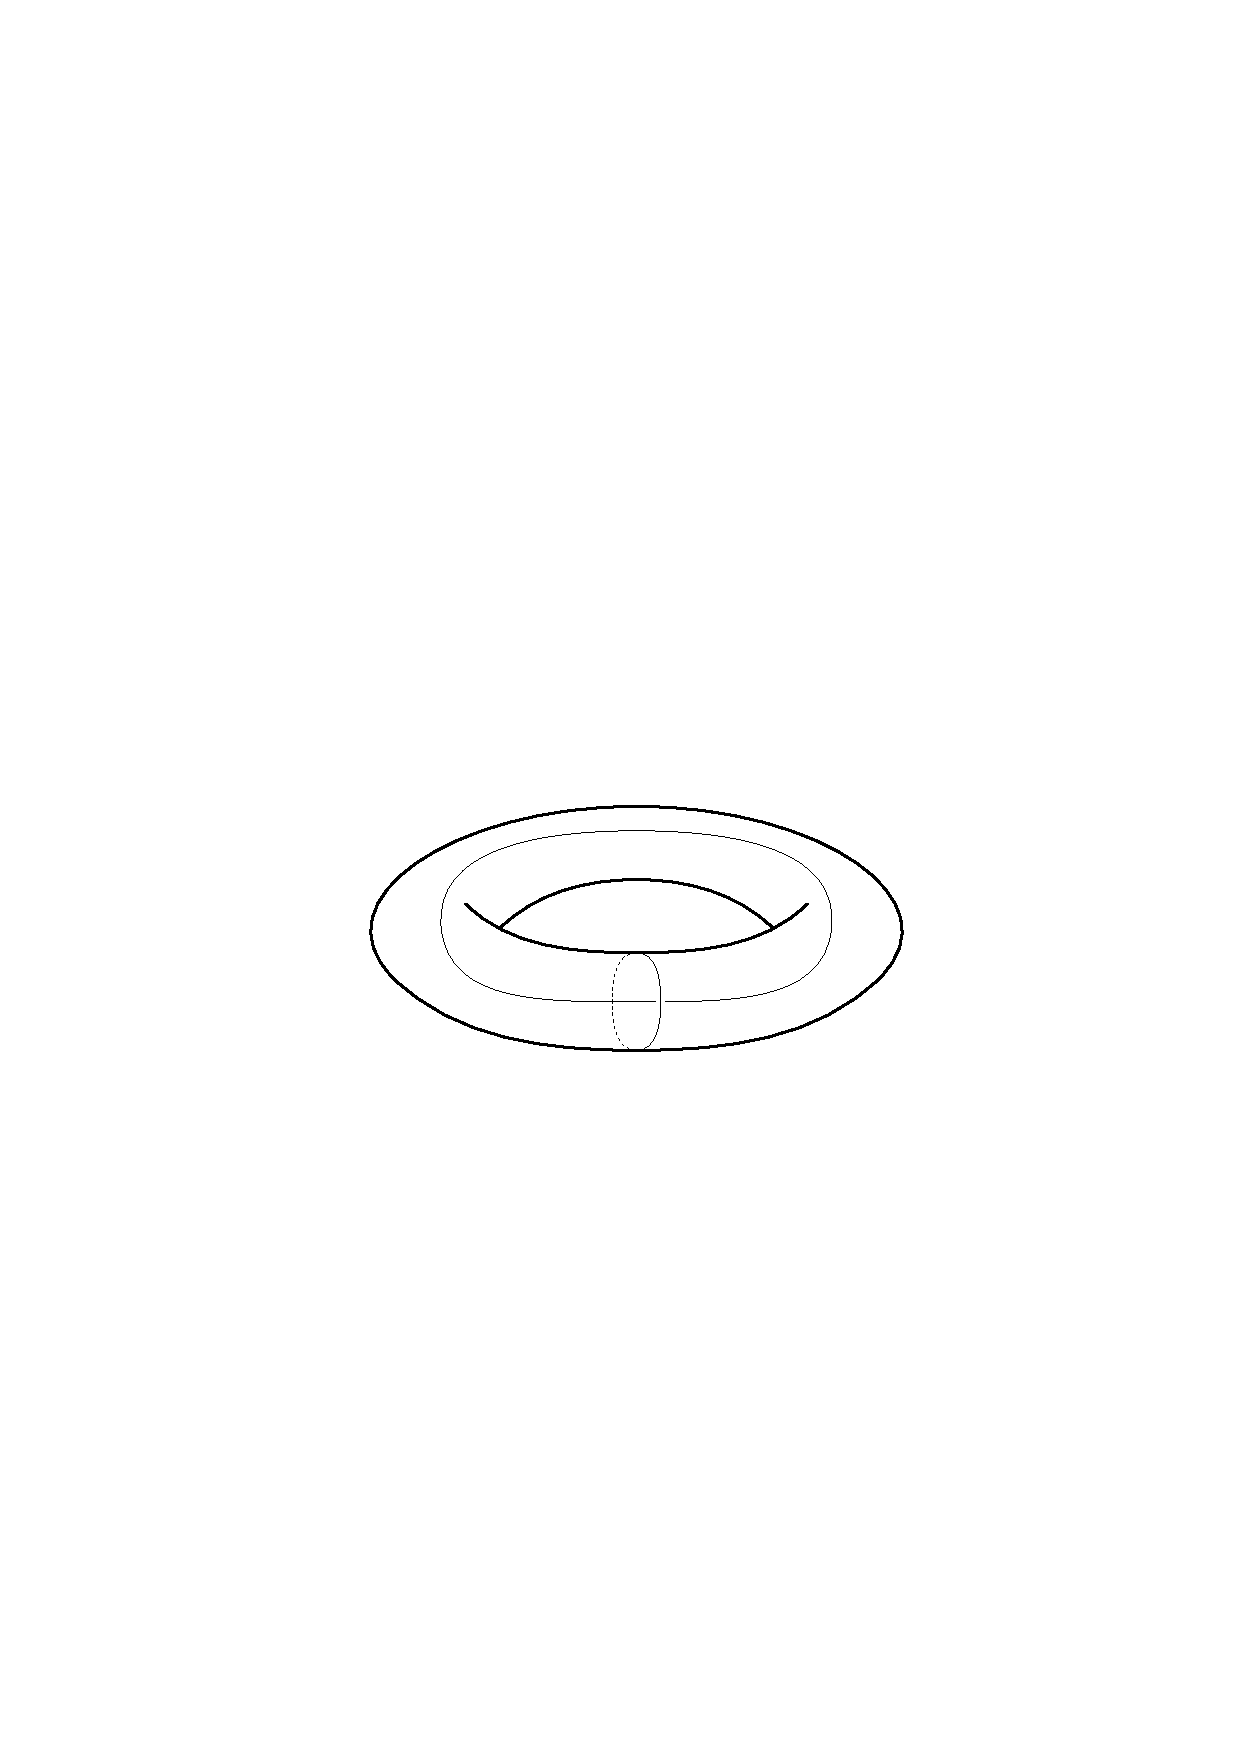
\includegraphics{chain_link_fence_knot_on_torus.pdf}
            \caption{Chain Link Fence Knot on a Torus}
            \label{fig:chain_link_fence_knot_on_torus}
        \end{figure}
        \par\hfill\par
        This last definition borrows the same difficulty from graph theory.
        While attaching handles at all of the $g$ virtual crossings yields an
        embedding into $M\times\mathbb{R}$ where $M$ is the compact orientable
        surface of genus $g$, it may have been possible to use fewer handles.
        Consider again Figs.~\ref{fig:graph_has_genus_001} and
        \ref{fig:graph_has_genus_002} where we created an embedding into the
        genus 3 compact surface. The starting graph was actually planar and
        need no additional handles (Fig.~\ref{fig:graph_has_genus_003}).
        \begin{figure}
            \centering
            \resizebox{0.5\textwidth}{!}{%
                \includegraphics{graph_has_genus_003.pdf}
            }
            \caption{Planar Embedding}
            \label{fig:graph_has_genus_003}
        \end{figure}
        \par\hfill\par
        While it is possible to compute the minimal genus of a virtual knot,
        we will not need such an algorithm. Our later work will be motivated
        by a more classical problem which is related to this difficulty.
        If one is given an extended Gauss code (a \textit{virtual knot}),
        is it possible to determine if there is a (classical) knot diagram
        that realizes this code? We can indeed do this in linear time.
        \par\hfill\par
        A valid Gauss code with $2N$ entries describes a virtual knot with
        $N$ crossings. Suppose we have embedded our virtual knot into
        $M\times\mathbb{R}$ where $M$ is a compact orientable surface of
        minimal genus. Projecting down the $\mathbb{R}$ component we obtain
        a graph embedded into $M$ where the crossings form the vertices. The
        graph is 4-valent, so by the hand-shaking theorem there are
        $2N$ edges. We are in effect decomposing $M$ into a CW complex with
        $N$ 0-cells, $2N$ 1-cells, and $F$ 2-cells. If we can compute $F$ we
        will obtain $g$ via Euler's formula:
        \begin{equation}
            V-E+F=2-2g
        \end{equation}
        Substituting $V=N$ and $E=2N$ we have:
        \begin{equation}
            g=\frac{2+N-F}{2}
        \end{equation}
        If we can compute $F$ we will have also computed $g$, and if
        $g\ne{0}$ we will know the extended Gauss code does not describe the
        knot diagram of a classical knot. We now describe how to compute $F$.
        \par\hfill\par
        \begin{figure}
            \centering
            \includegraphics{thickened_crossings.pdf}
            \caption{Signed Thickened Crossings}
            \label{fig:thickened_crossings}
        \end{figure}
        Thicken the knot projection so that the crossings look like
        Fig.~\ref{fig:thickened_crossings}. Begin traveling along the thickened
        knot, following the orientation given by the Gauss code, and place your
        finger on the left wall at all times. When you come to a crossing,
        turn left so that your finger remains continuously on the wall of the
        thickened knot. Continue doing this until you return to your starting
        point. You will have just traced out a $k$-gon for some
        $k\in\mathbb{N}$. Attach a 2-cell by gluing along this polygon.
        Continue doing this until all $4N$ of the corners of the thickened
        crossings (again, appeal to Fig.~\ref{fig:thickened_crossings}) have
        be traveled. The total number of faces, which is the total number of
        cycles you've traveled, has now been computed. We require $4N$ steps,
        and so our algorithm does indeed run in linear time.
        \par\hfill\par
        The steps described translate to jumping between the entries in the
        Gauss code in a well-defined manner. \textit{Going left} means changing
        crossing type and then walking with or against the orientation.
        That is, if you come to entry \texttt{Ons}, with \texttt{n} the index
        and \texttt{s} the sign, jump ahead to \texttt{Uns}, changing crossing
        type. You then proceed to either the next entry in the Gauss code or
        the previous entry depending on the value of the sign \texttt{s}.
        This amounts to walking forwards or backwards. The correct direction
        can be computed from Fig.~\ref{fig:thickened_crossings}. If you are at
        the final entry and need to proceed forward, loop back around to the
        start. Similarly, if you are at the starting entry and need to move
        backwards, jump ahead to the end of the Gauss code. By repeatedly
        doing this we can compute the number of cycles and consequently
        calculate the genus.
        \par\hfill\par
        Applying this algorithm to the standard 3-crossing trefoil (either the
        left handed or right handed) will yield 5 faces, giving us a genus of
        0. The chain link fence knot \texttt{O0+ U1+ U0+ O1+} produces 2 faces,
        and so we end up with a genus 1 knot diagram which can be embedded on
        the torus. The faces, and the reason for the name
        \textit{chain link fence}, can be easily seen if we conduct our drawings
        on the flat torus (Fig.~\ref{fig:chain_link_fence_knot_on_flat_torus}).
        If we lift to the universal cover of the torus, which is the Euclidean
        plane, we can see the two aforementioned faces, as well as a chain
        link fence pattern
        (Fig.~\ref{fig:chain_link_fence_knot_on_flat_torus_universal_cover}).
        \begin{figure}
            \centering
            \includegraphics{chain_link_fence_knot_on_flat_torus.pdf}
            \caption{Chain Link Fence Virtual Knot on a Flat Torus}
            \label{fig:chain_link_fence_knot_on_flat_torus}
        \end{figure}
        \begin{figure}
            \centering
            \resizebox{\textwidth}{!}{%
                \includegraphics{%
                    chain_link_fence_knot_on_flat_torus_universal_cover.pdf
                }
            }
            \caption{Lift of the Chain Link Fence to the Universal Cover}
            \label{fig:chain_link_fence_knot_on_flat_torus_universal_cover}
        \end{figure}
        \par\hfill\par
        It should be considered a pleasant bonus if a knot invariant is also
        an invariant for virtual knots. It is especially enjoyable when an
        algorithm for a knot invariant can be copied for virtual knots with
        little or no additional effort. But, before proceeding, two warnings
        are worth mentioning.
        \par\hfill\par
        The operations of the Reidemeister moves are stricter for virtual knots
        via extended Gauss code. For classical knots, should we find
        \texttt{On Om} followed by \texttt{Un Um}, or any re-ordering thereof,
        we can apply Type II and delete the four entries from the code. This is
        not so for virtual knots. Indeed, were it true the chain link fence
        would be equivalent to the unknot. The sign is crucial for a correct
        description of Type II moves in the virtual setting. For a true
        Type II move, the signs alternate. This in agreement with the fact that
        Type II does not change the writhe of a diagram. So, should we find
        \texttt{On+ Om-} followed by \texttt{Un+ Um-}, or any re-ordering
        thereof, we may apply Type II and delete the four entries, be it a
        classical or virtual knot.
        \par\hfill\par
        Lastly, the algorithm described previously computed the genus of a
        virtual knot \textit{diagram}, and not the minimal genus of all
        possible equivalent diagram. By application of Type II it is possible
        give the right-handed trefoil a genus 1 knot diagram, for example
        \texttt{O0+ U1+ O2+ O3- O4+ U0+ U3- U2+ O1+ U4+}. The Reidemeister
        moves may change the genus of a diagram.
    \subsection{Planar Diagrams}
        Planar diagram code, commonly called PD code, is one of the more popular
        representations found in programming libraries. We start with an
        oriented knot diagram and pick a starting point. We follow the
        orientation and label the \textit{arcs}, the edges between crossings,
        in increasing order from $0$ to $2N-1$ where $N$ is the number of
        crossings. Once the arcs have been labeled we once again walk around
        the knot diagram and each time we come across an under crossing we write
        down \texttt{X[a,b,c,d]} where \texttt{a} is the number of the arc you
        are coming from, \texttt{c} is the arc you'll be leaving through,
        \texttt{b} is the arc to your \textit{right}, and \texttt{d} is the
        arc to your \textit{left}. The PD code of the diagram is the ordered
        sequence of 4-tuples \texttt{X[a,b,c,d]} for each under crossing you
        encounter in the order you encounter them. Using
        Fig.~\ref{fig:trefoil_knot_arcs_labeled}, the right-handed trefoil can
        represented by writing \texttt{X[1,5,2,4],X[3,1,4,0],X[5,3,0,2]}.
        \begin{figure}
            \centering
            \includegraphics{trefoil_knot_arcs_labeled.pdf}
            \caption{Trefoil Knot with Arcs Labeled}
            \label{fig:trefoil_knot_arcs_labeled}
        \end{figure}
        \par\hfill\par
        Planar diagram code can recover unsigned Gauss code, but moreover
        the sign of the crossings can also be computed. Since the arcs are in
        increasing order, we have that for each entry
        \texttt{X[a,b,c,d]}, the difference $\texttt{c}-\texttt{a}$ is either
        1 or $1-N$, with $1-N$ occurring if and only of \texttt{a} is the final
        arc in the ordering. In contrast, the difference $\texttt{d}-\texttt{b}$
        can be $+1$ or $-1$, once reduced mod $N$. $+1$ means the crossing is
        positive and $-1$ means the crossing is negative. Whether this is a
        lucky coincidence, or if the signing of the crossings was originally
        chosen to yield this result, one must admit it is a rather elegant
        computation.
        \par\hfill\par
        Since the signs of the crossings can be computed, and since
        PD code can determine the unsigned Gauss code, we immediately see that
        PD code and extended Gauss code have the same information. Because of
        this one may use PD codes for virtual knots as well, but the phrasing
        \textit{virtual planar diagram code} is rather unfortunate for
        non-planar virtual knot diagrams. At any rate, it is \textit{not}
        common practice to use PD codes to represent virtual knots. Indeed,
        some programming libraries have checks to ensure the input PD code
        represents a planar knot diagram before allowing computations to be
        performed.
    \subsection{Dowker-Thistlethwaite Notation}
        Dowker-Thistlethwaite code (DT code for short) compactly describes
        knots. Because of this it is used in tabulation efforts where millions
        of distinct knot are listed in massive tables
        (see, for example \cite{Burton2020TheN3} and \cite{regina}).
        \par\hfill\par
        Start with an oriented knot diagram and choose a starting point.
        Walk along the knot, following the orientation, and number the
        crossings as you pass them in increasing order. For each odd number,
        if you are on the under strand as you pass the crossing,
        prepend a minus sign. Should you come upon a crossing you've already
        marked, label it again with the second number second number as well.
        At the end you should have a permutation of all numbers (with possible
        minus signs) between $0$ and $2N-1$ where $N$ is the number of
        crossings, each crossing having two numbers assigned to it. If the knot
        diagram is \textit{planar} and represents a classical knot, by a
        parity argument and the Jordan curve theorem we see that each crossing
        will have one odd number and one even number associated to it. Pair
        the numbers together into tuples $(2n,\,\pm{2m+1})$ corresponding to the
        same crossing. Lastly, order the tuples lexicographically by giving
        preference to the first entry (the even number in the tuple).
        The DT code is the corresponding ordered sequence of even numbers,
        with minus signs included.\footnote{%
            In computer science it is very common to start numbering at zero,
            which is what we have done several times throughout. In the
            original paper the labeling start at 1. Because of this the
            \textit{even} numbers are given plus and minus signs, and the
            tuples are ordered with respect to the \textit{odd} numbers. A
            minor change, but a very important one. Failure to be consistent
            can result in the wrong DT code!
        }
        \par\hfill\par
        Quite verbose, let us consider an example.
        Fig.~\ref{fig:trefoil_knot_oriented_001} depicts an oriented
        right-handed trefoil, let's start with this. Choosing the top-most
        point, we obtain the sequence of ordered tuples
        $(0,\,3)$, $(2,\,5)$, $(4,\,1)$. So our DT code for the right-handed
        trefoil is \texttt{3 5 1}. The same DT code is attainable for the
        left-handed trefoil, meaning the notation is mirror insensitive. Still,
        it is extremely compact. The following theorem further justifies its
        use.
        \begin{theorem}[Dowker, Thistlethwaite 1983]
            If two prime knots have the same DT code, then they are either
            equivalent or are mirrors of one another.
        \end{theorem}
        \begin{proof}
            See \cite{DOWKER198319}.
        \end{proof}
        Since knot tabulation rarely differentiates between mirrors, and
        almost exclusively concerns itself with the listing of prime knots,
        DT code is perfect for such an endeavor.
        \par\hfill\par
        Since the code consists entirely of odd numbers we can obtain the
        \textbf{simplified DT code} by subtracting one and dividing by two,
        doing this to each element. The trefoil then becomes
        \texttt{1 2 0}. Furthermore, should we be concerned with knots of
        no more than 26 crossings, we can substitute numbers with letters.
        This is the \textbf{alphabetical DT code}. The trefoil becomes
        \texttt{bca}. Should a minus sign be part of the original DT code
        we would add one and divide by two for the simplified code, and the
        alphabetical code would be given using a capital letter. For example,
        the knot $8_{19}$ in the Rolfsen table
        has the alphabetical DT code
        \texttt{bdFaGHCE}. In our presentation of knot tables we will
        exclusively use the alphabetical DT notation for its brevity.
    \subsection{Braids}
        Braids are one of the original means of representing knots
    \subsection{Tangles}
    \subsection{Tait Graphs}
